\documentclass[graphics]{beamer}
\usepackage{xcolor}
\usepackage{graphicx}
\usepackage{verbatim}
\usepackage{wrapfig}
\usepackage{tabularx}
\usepackage{multirow}
\usepackage{amssymb}
\usepackage{pifont}
\usepackage{tikz}
\def\Checkmark{\tikz\fill[scale=0.2](0,.35) -- (.25,0) -- (1,.7) -- (.25,.15) -- cycle;} 

\useoutertheme{shadow}
%\usecolortheme{orchid}
\usecolortheme{seahorse}
\newcommand{\cmark}{\text{\ding{51}}}
%\newcommand*{\GtrSim}{\smallrel\gtrsim}

% math commands
\newcommand{\be}{\begin{eqnarray}}
\newcommand{\ee}{\end{eqnarray}}
\newcommand{\beq}{\begin{equation}}
\newcommand{\eeq}{\end{equation}}
\def\simless{\mathbin{\lower 3pt\hbox
      {$\rlap{\raise 5pt\hbox{$\char'074$}}\mathchar"7218$}}}
\def\simgreat{\mathbin{\lower 3pt\hbox
      {$\rlap{\raise 5pt\hbox{$\char'076$}}\mathchar"7218$}}} %> or of order

% variables

\def\toonscale{0.45}
\def\mboxy#1{\mbox{\small #1}}

\defbeamertemplate*{title page}{customized}[1][]
{
  \usebeamerfont{title}\inserttitle\par
  \usebeamerfont{subtitle}\usebeamercolor[fg]{subtitle}\insertsubtitle\par
  \bigskip
  \usebeamerfont{author}\insertauthor\par
  \usebeamerfont{institute}\insertinstitute\par
  \usebeamerfont{date}\insertdate\par
  \usebeamercolor[fg]{titlegraphic}\inserttitlegraphic
}
\begin{comment}
\AtBeginSection[]{
  \frame{
    \frametitle{Outline}
    \tableofcontents[currentsection]
  }
}
\end{comment}


\title{\textcolor{white}{Nano-arcsecond pulsar mapping}}
%\subtitle{}
\author[U. Pen]{{
\textcolor{green}{\small Ue-Li Pen, CITA, scintillometry collaboration}
}
\\[8mm] 
}
\date{\textcolor{green}{March 17, 2017}}


\begin{document}

\frame{
\vspace{-0.5in}
\begin{center}  
%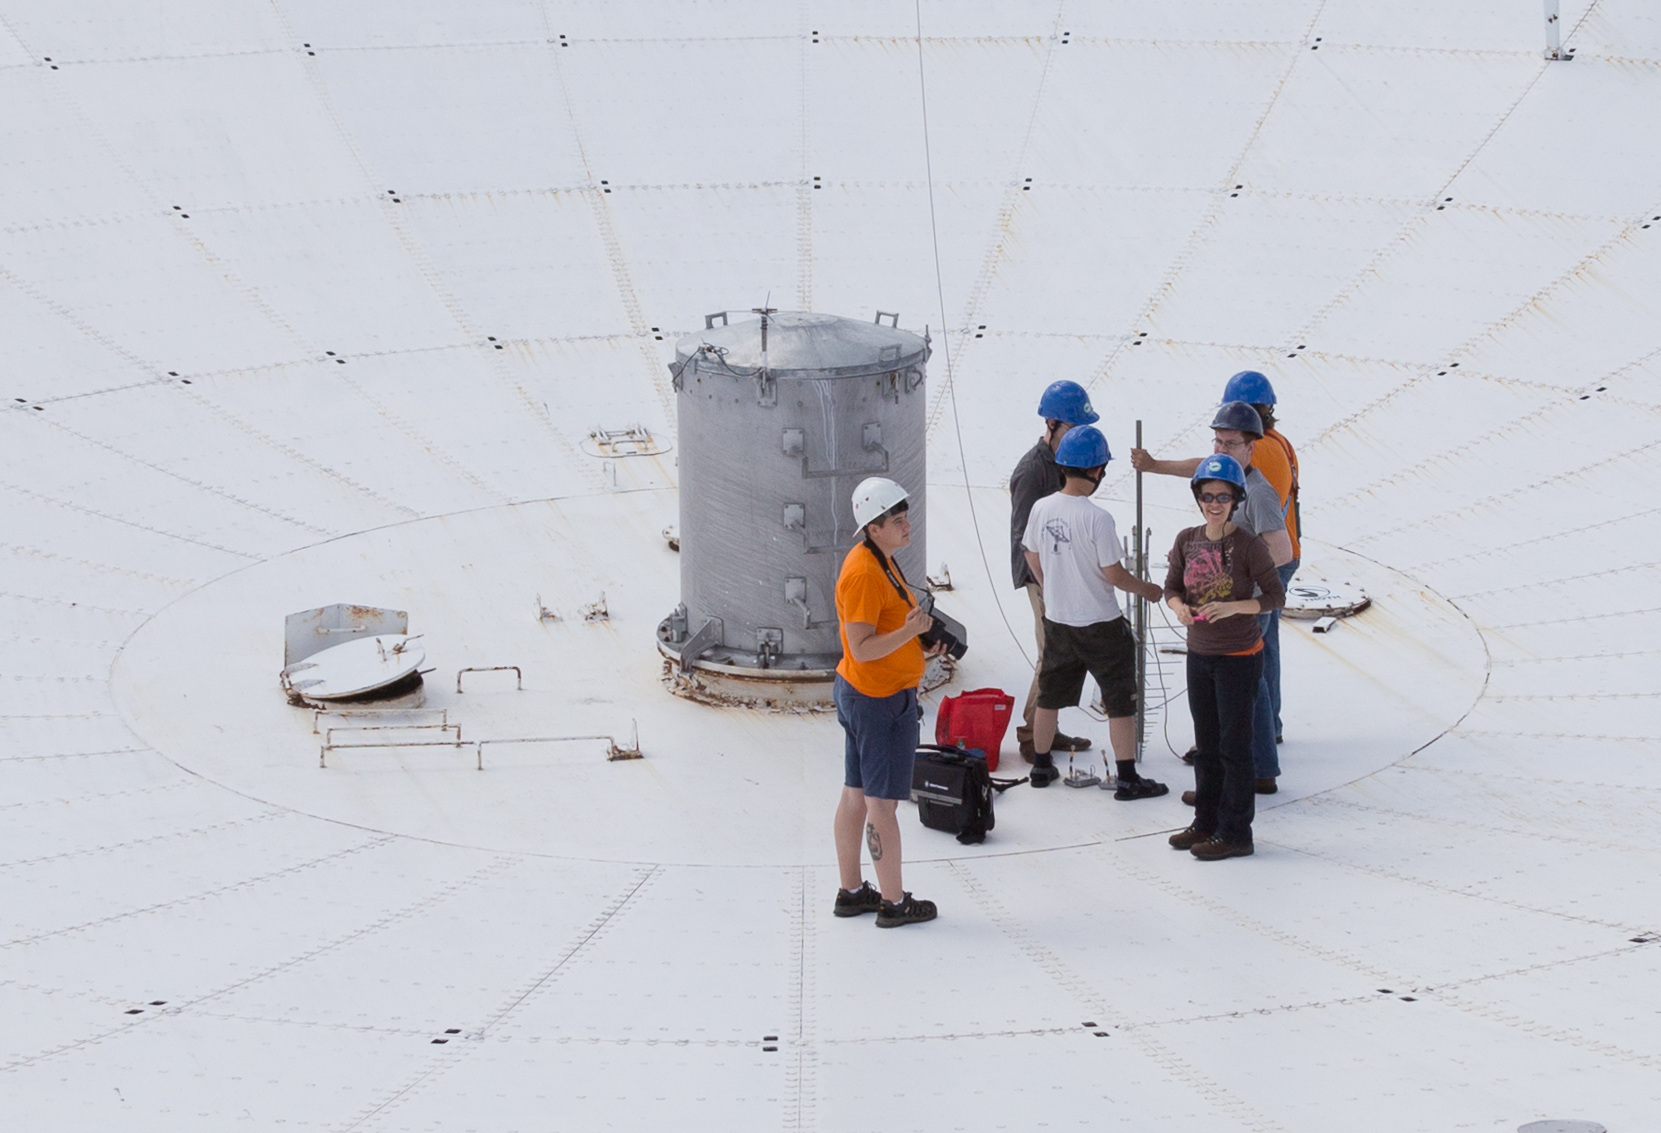
\includegraphics[width=4.4in]{Figures/IMG-0438-by-Andre-cropped.jpg}
\end{center}
\begin{picture}(320,250)
\put(-35,6){
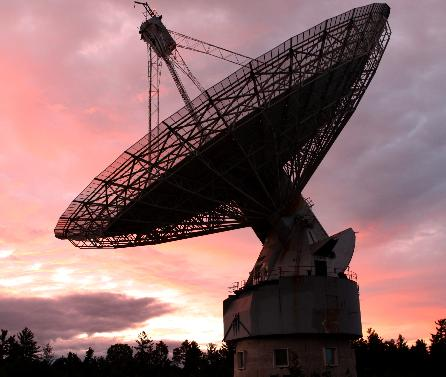
\includegraphics[width=5.1in]{Figures/IMG-7749-ARO-crop.JPG}
}
\end{picture}
\vspace{-4in}
\\
%image credit: NRAO/AUI/NSF
\\
\vspace{1in}
\titlepage
}

%\section*{Introduction}
\section{Introduction}

\begin{comment}
  \subsection{Outline}

  \frame{
    \frametitle{Outline}
    \tableofcontents
  }
\end{comment}

  \frame{
    \frametitle{Overview}
    \begin{itemize}
      \item Half century of VLBI and pulsars -- beginning of pulsar-VLBI
      \item Plasma telecopes
      \item tower of telescopes
      \item crab at the tip of the pyramid
    \end{itemize}
  }


\frame{
    \frametitle{VLBI of lenses}
     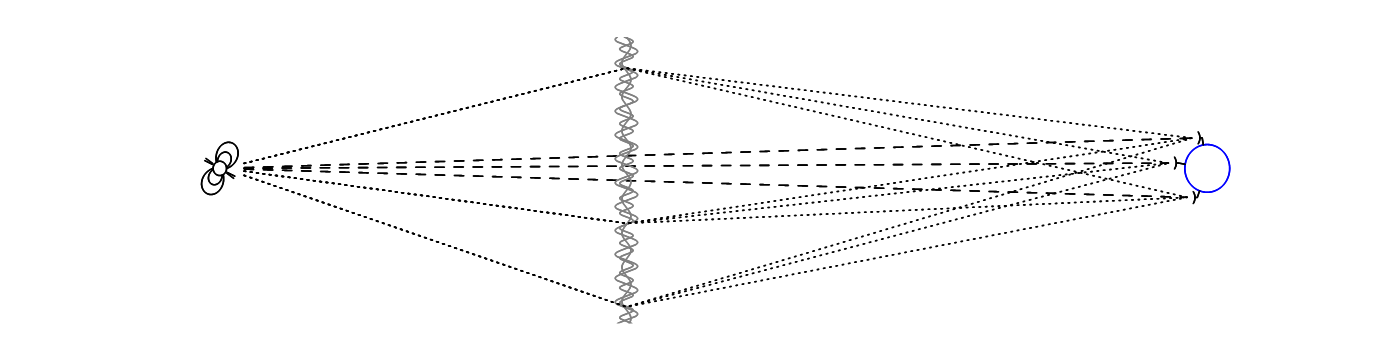
\includegraphics[width=1.1\textwidth]{Figures/scint-schematic.png}

(figure credit: M. van Kerkwijk)
}


  \frame{
    \frametitle{Scintillometry}
PSR B0834+06: 

$D_S=620$pc, 

$D_L=389/415$pc

{\tiny Brisken+2010, Liu+2016}
\begin{picture}(320,250)
\put(110,90){
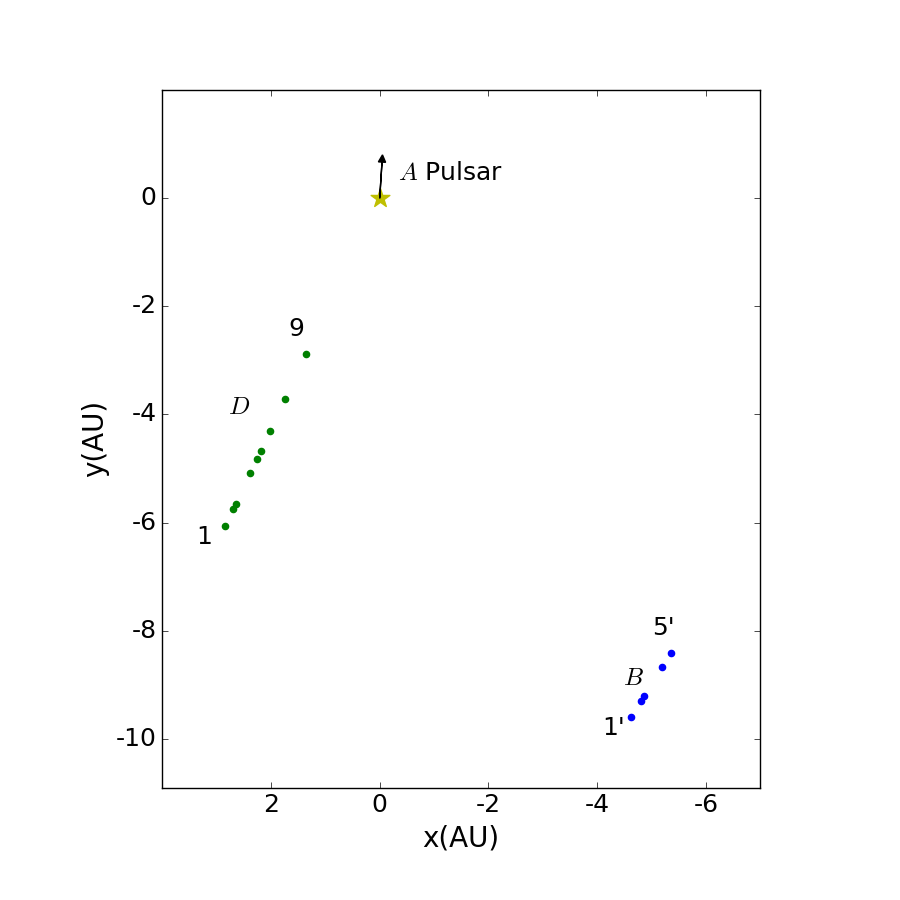
\includegraphics[width=0.7\textwidth]{Figures/Fig7_without_lines_5.png} 
}
\end{picture}
%\vspace{-4in}

  }



\frame{
    \frametitle{Crab}
     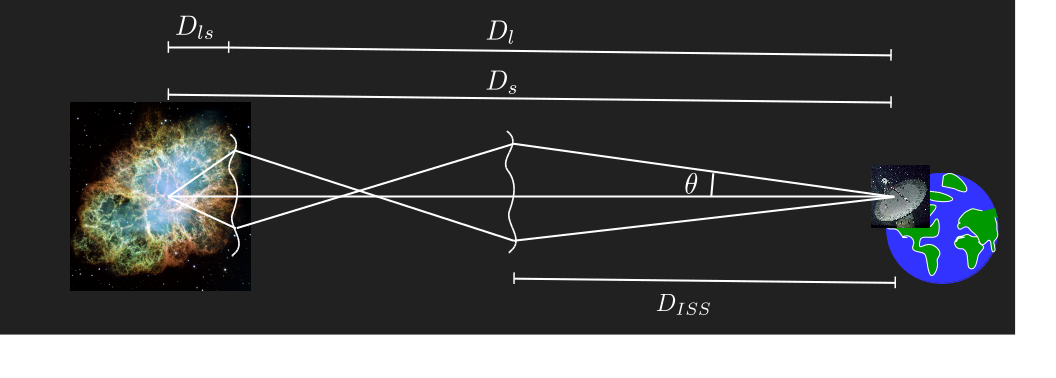
\includegraphics[width=1.1\textwidth]{Figures/TwoScreenGeometry.png}

(figure credit: R. Main)
}



  \frame{
    \frametitle{Crab data}
    \begin{itemize}
      \item VLBI measurements from 0.15 to 2+ GHz
      \item interstellar screen resolved
      \item circum pulsar screen resolved by ISM screen about 2GHz
      \item pulsar screen resolves main-pulse vs interpulse at 1.4 GHz
      \item individual components resolved at 800 MHz
      \item able to test Philippov scenario of coherent emission from
        outside the light cylinder!
    \end{itemize}
  }



\frame{
    \frametitle{MP Scintillation Correlations}
     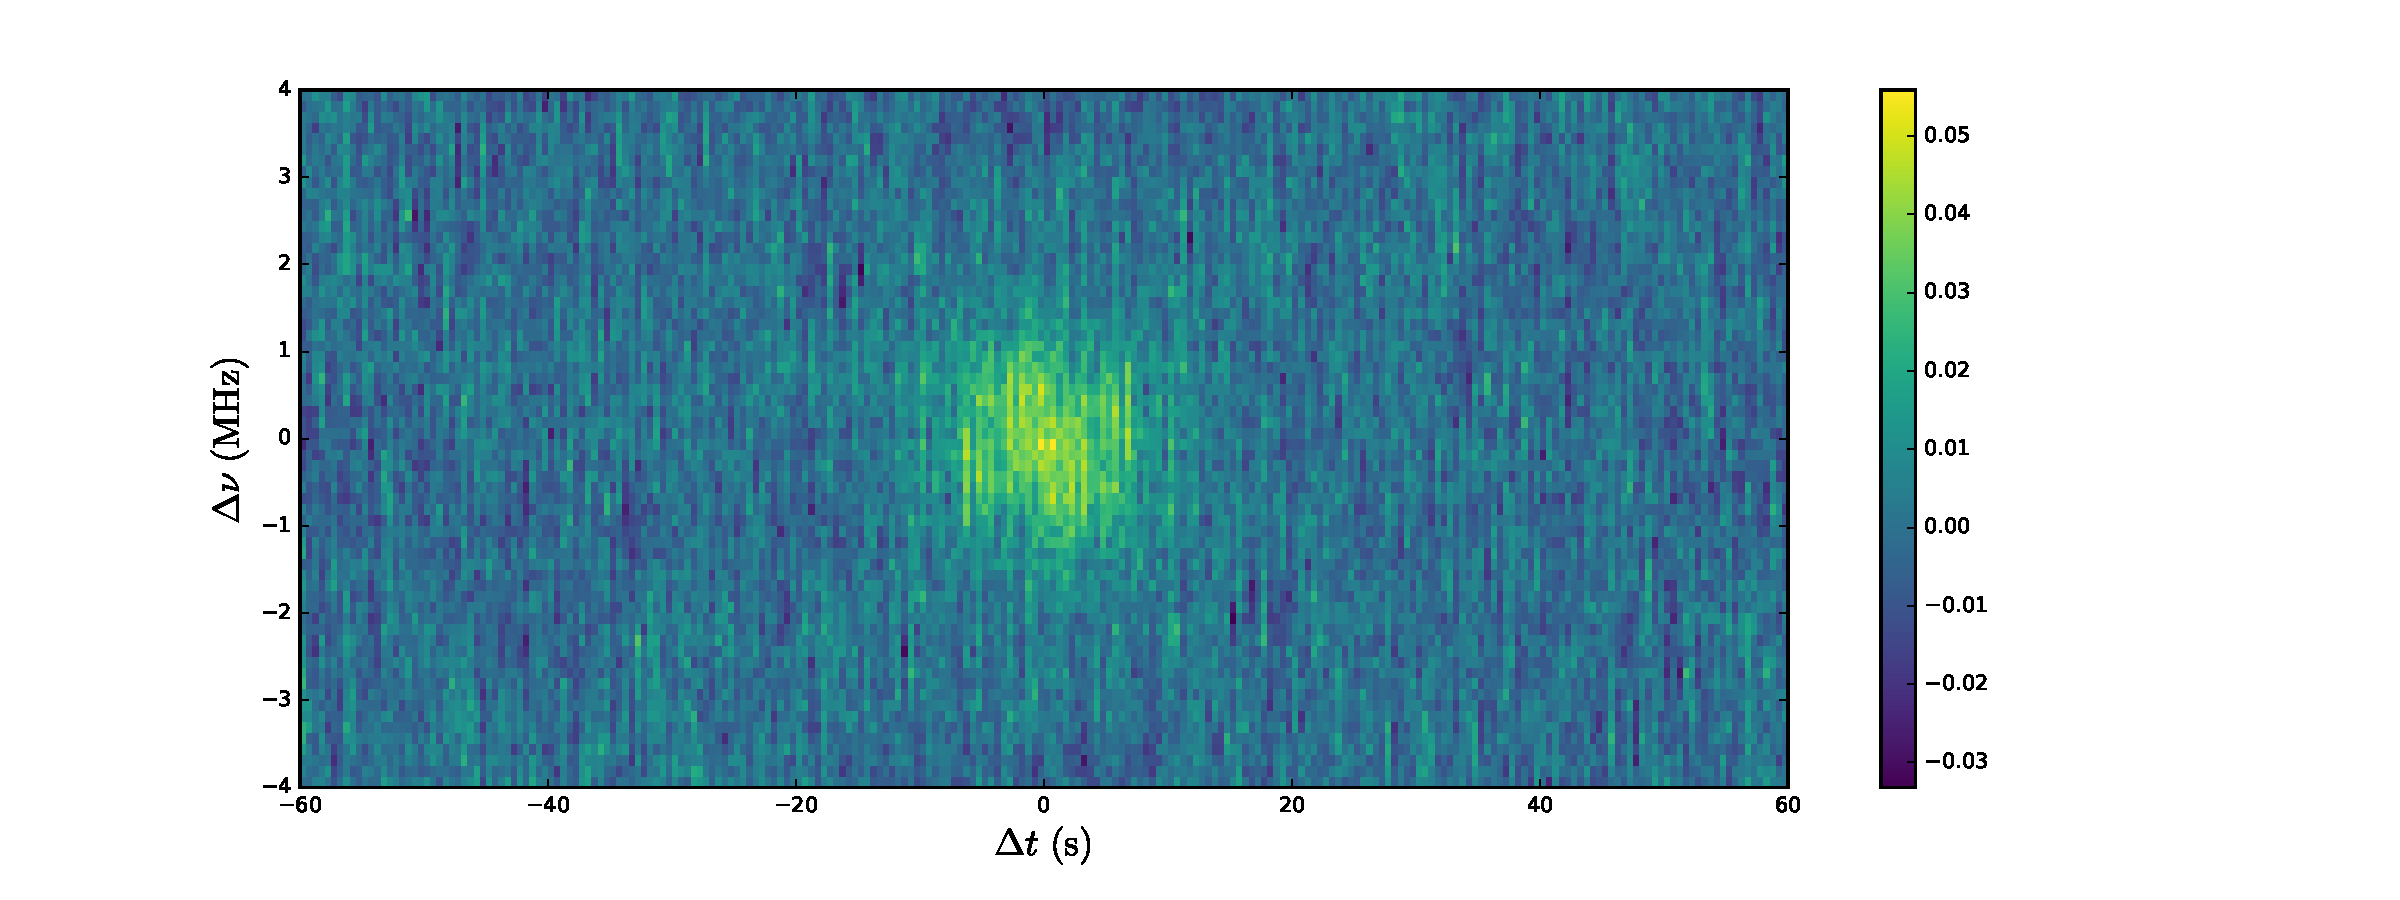
\includegraphics[width=1.3\textwidth]{Figures/MP-MP-ccorr.pdf}

 Main et al in prep
}

\section{Summary}



  \frame{
    \frametitle{Conclusion}
    \begin{itemize}
      \item localized interstellar plasma lenses supercede outdated turbulence picture.
      \item interstellar plasma lenses act as interferometer to map
        pulsar emission
      \item circum pulsar nebula act as additional lens
      \item ISM lens sometimes resolves nebula lens
      \item also works for FRB's
      \item systematic study of pulsar magnetospheres with pulsar VLBI
      \item promising future with CHIME, ARO, GMRT, LOFAR, etc.
    \end{itemize}
  }

\end{document}
